
\section{Quantitative Results}

\begin{figure}[htbp]
\centering

\begin{subfigure}{1\textwidth}
    \centering
    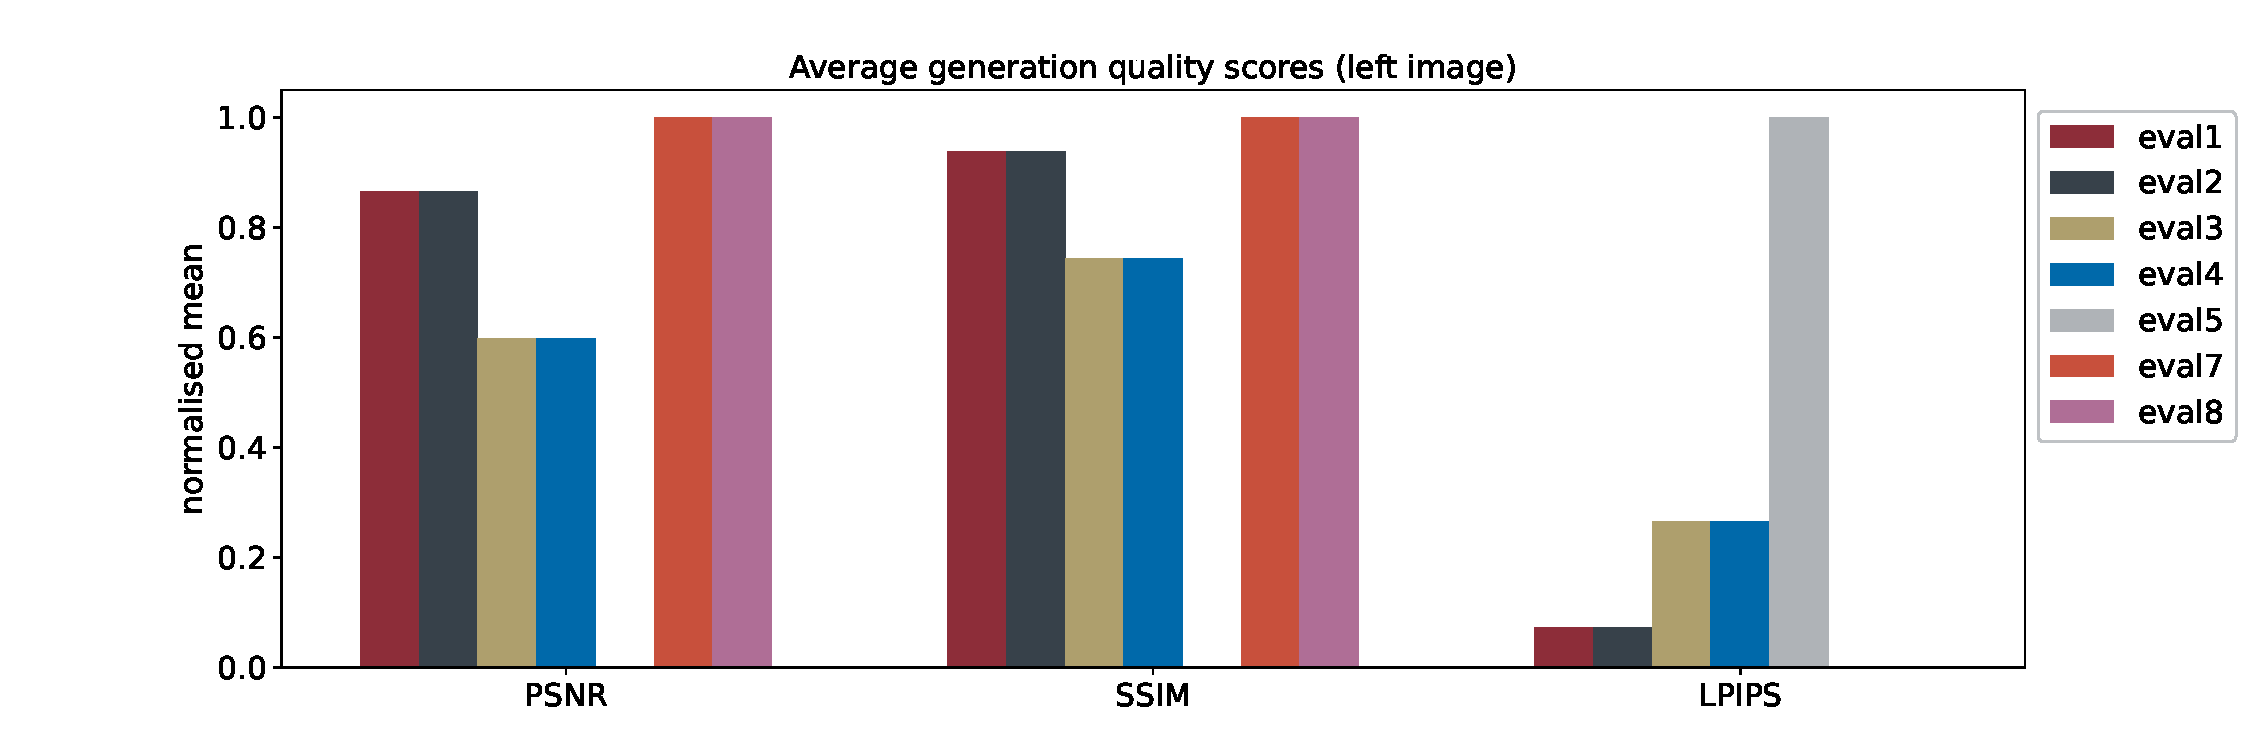
\includegraphics[width=\linewidth]{figures/eval_quality_left_mean.pdf}
    \caption{Average scores (left image)}
\end{subfigure}


\hfill
\begin{subfigure}{1\textwidth}
    \centering
    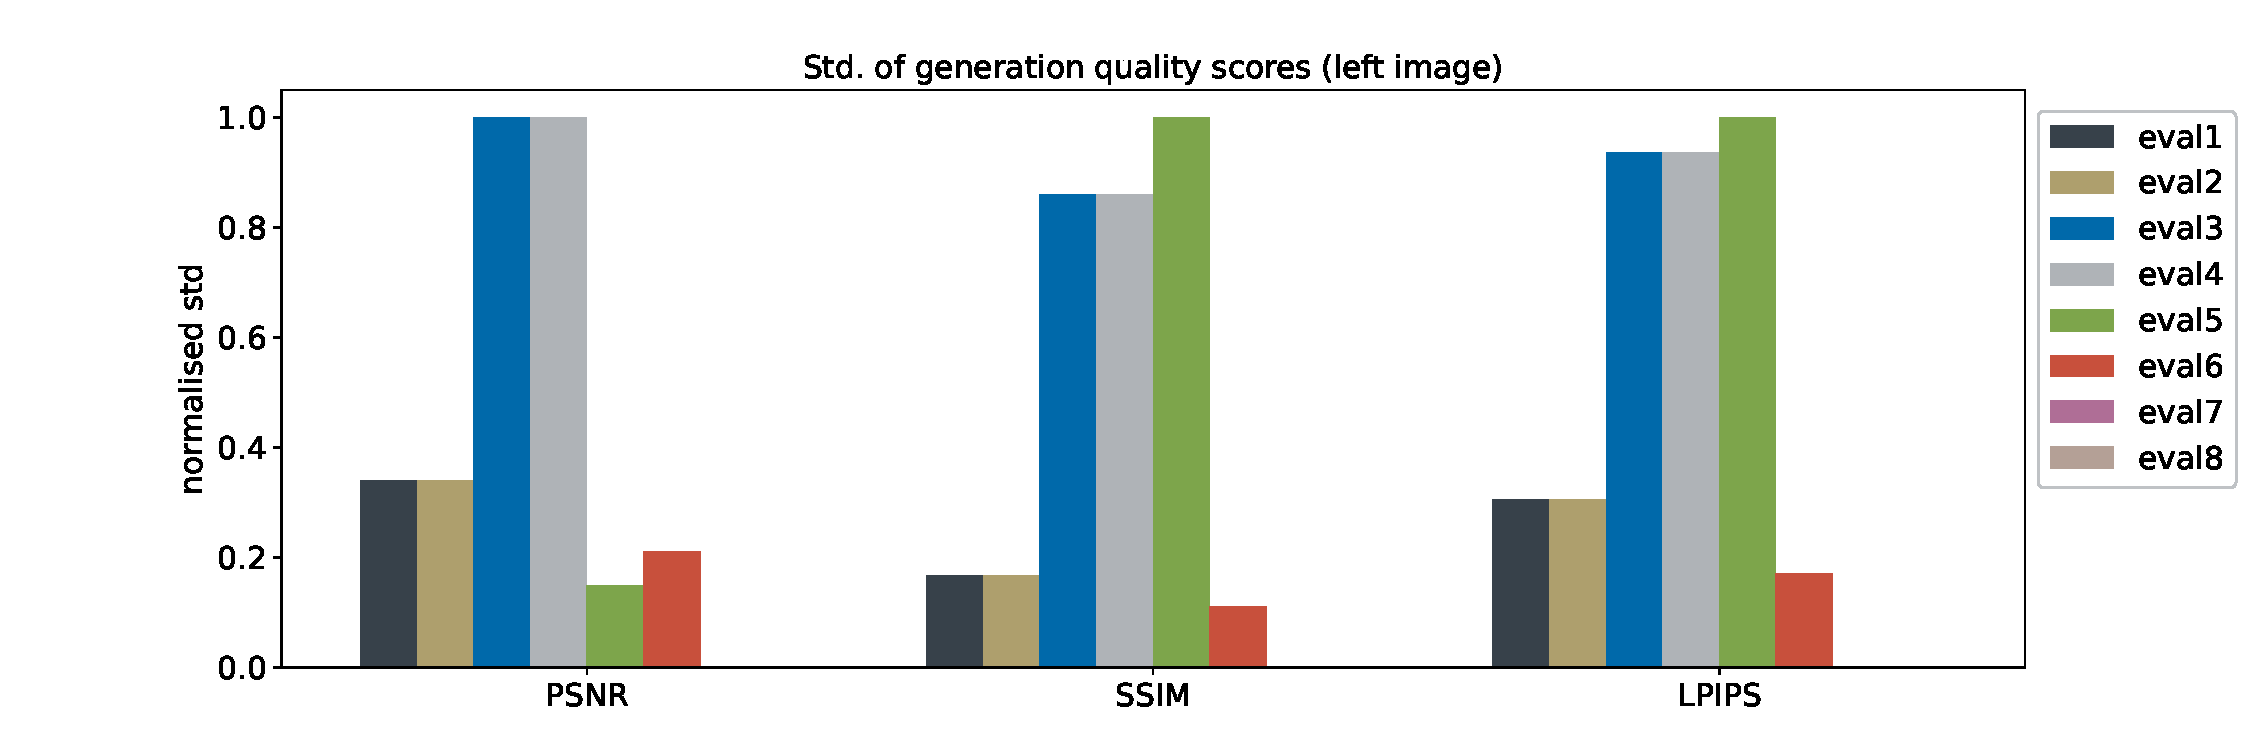
\includegraphics[width=\linewidth]{figures/eval_quality_left_std.pdf}
    \caption{Standard deviation (left image)}
\end{subfigure}

\vspace{0.5cm}

\begin{subfigure}{1\textwidth}
    \centering
    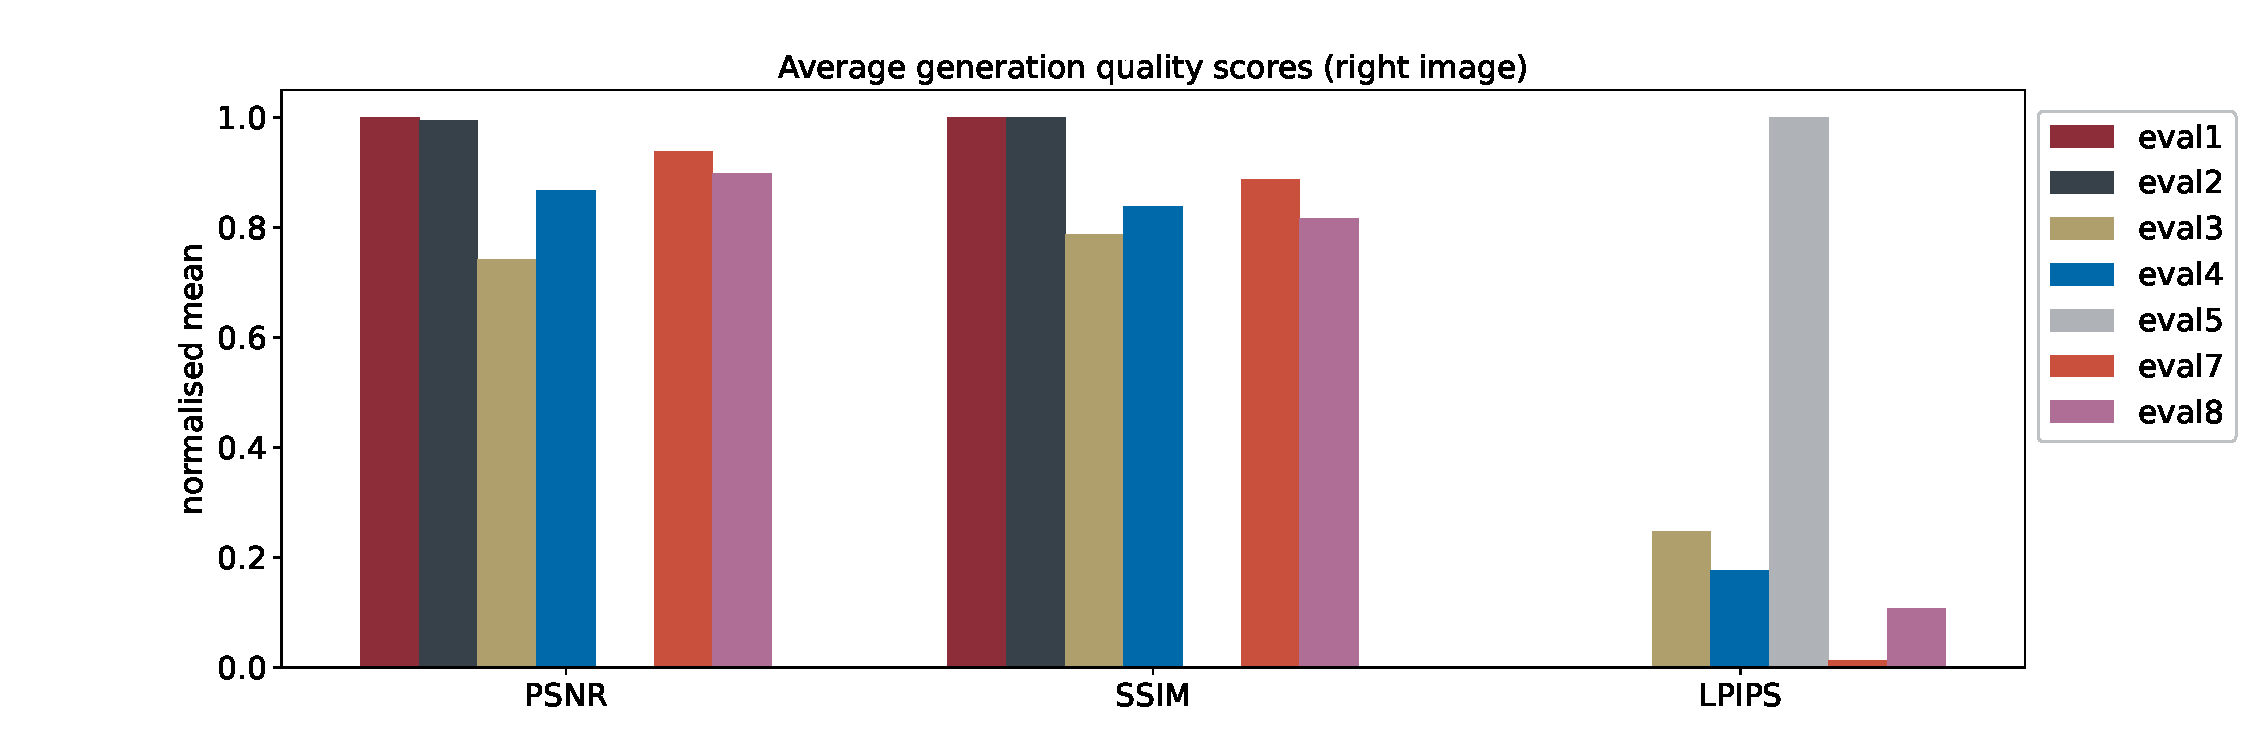
\includegraphics[width=\linewidth]{figures/eval_quality_right_mean.pdf}
    \caption{Average scores (right image)}
\end{subfigure}
\hfill
\begin{subfigure}{1\textwidth}
    \centering
    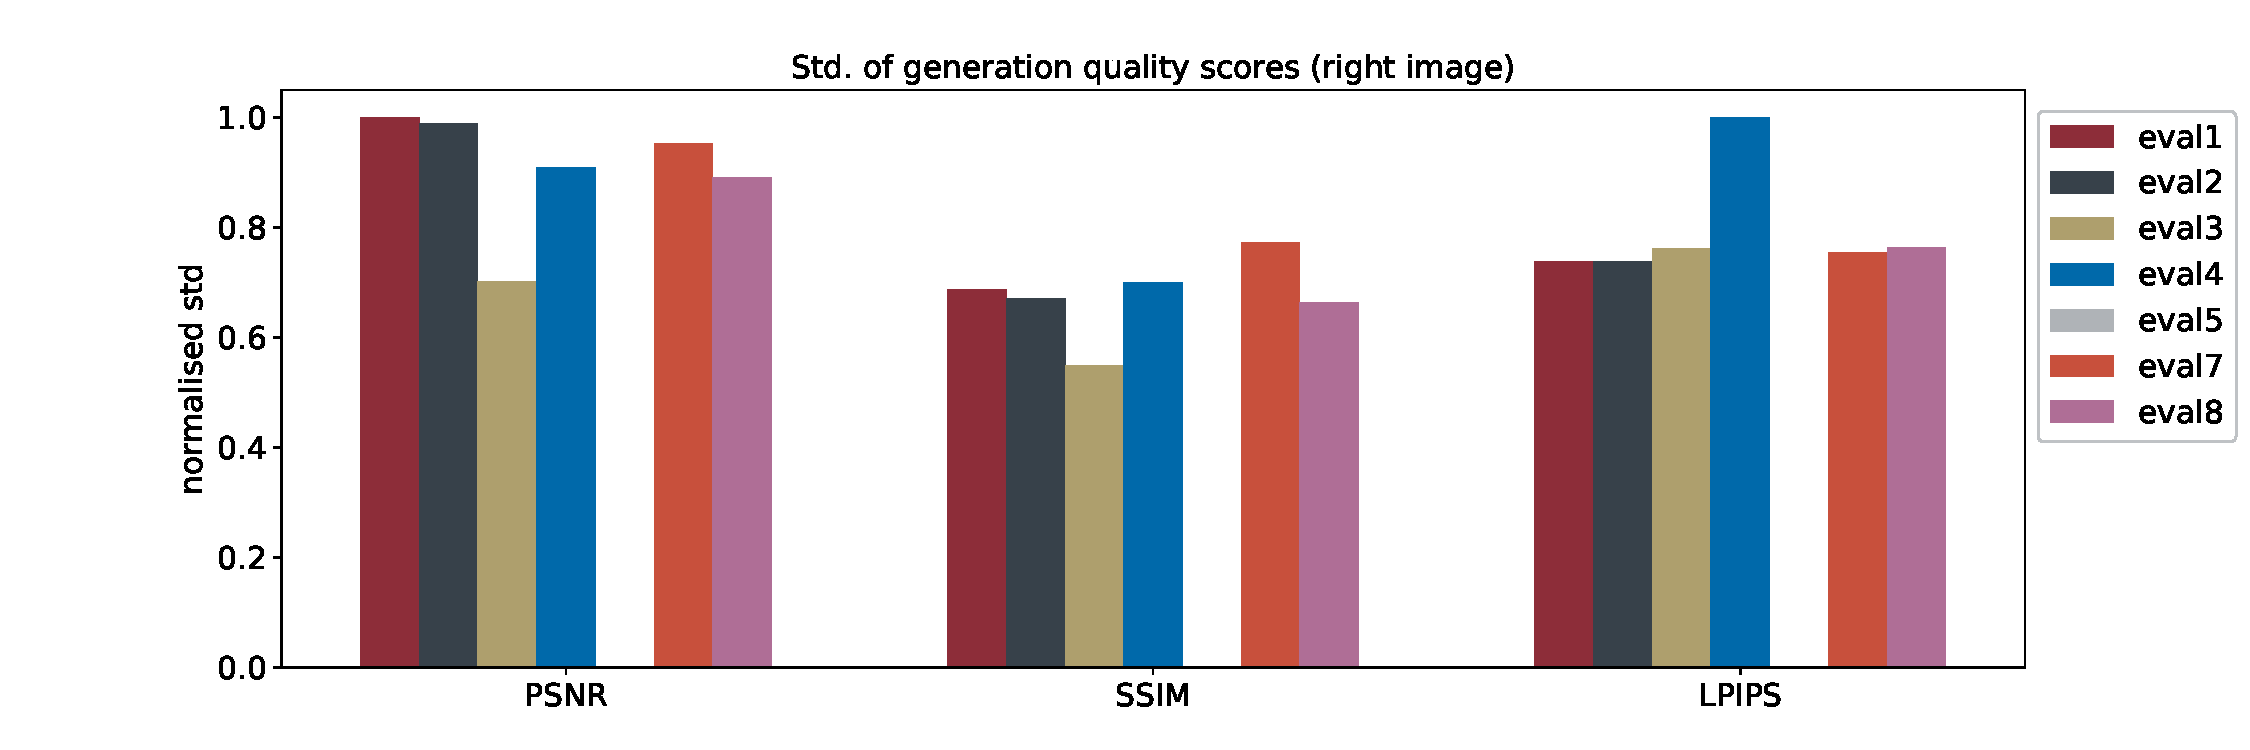
\includegraphics[width=\linewidth]{figures/eval_quality_right_std.pdf}
    \caption{Standard deviation (right image)}
\end{subfigure}

\caption{\textbf{Quantitative evaluation of stereo generation quality.} 
Comparison of PSNR, SSIM, and LPIPS across different evaluation configurations. 
Top(a and b): left image results; bottom(c and d): right image results. 
Mean values indicate overall performance, while standard deviation reflects stability across samples. 
Lower LPIPS and higher PSNR/SSIM correspond to better quality.}
\label{fig:quantitative_results}

\end{figure}

We evaluate the quality of generated stereo images via PSNR, SSIM, and LPIPS. These metrics represent the pixel-wise accuracy, the structure of the image, and the percptual quality. Table 1 provides an overview of all the results obtained through all possible configurations. The best performance was obtained by the baseline configuration (Eval1) which follows closely the original StereoDiffusion configuration. With respect to the right view, this configuration reaches the highest reconstruction quality among all evaluated variants (19.16 PSNR, 0.618 SSIM, and 0.106 LPIPS).
Replacing the disparity with a depth-to-disparity estimate (Eval2) yields similar results (PSNR 19.15, SSIM 0.618, LPIPS 0.106), thus showing that a depth based approach to compute disparities may be used without affecting the quality of the reconstructed stereo images. On the other hand, when including a conditional prompt, there is a consistent degradation in terms of performance. For instance, Eval3 (with prompt+cross-attention) resulted in PSNR=18.67, SSIM=0.601, and LPIPS =0.126. In contrast, Eval4 (with prompt + uni-directional attention) yielded better results but inferior compared to the default configuration (PSNR = 18.91 and LPIPS = 0.120). The worst performance was observed for Eval5 (with bi-directional attention) which presented a huge reduction in terms of PSNR to 17.27 and a huge increase in LPIPS to 0.186, revealing important degradation both at the structural level and at the perceptive level.
Furthermore, these results confirm that uni-directional attention is more stable than cross-attention or bi-directional attention. The performance gap between Eval4 (uni-directional) and Eval5 (bi-directional) illustrate how more complex attention mechanisms can negatively affect geometric coherence in a training-free setting.
Finally, ground truth alignment (Eval7 and Eval8) produces results close to those of the default configuration. Here Eval7 achieves PSNR = 19.04, SSIM = 0.609, and LPIPS = 0.107 while Eval8 exhibits slightly worse performance with PSNR = 18.97 and LPIPS = 0.114. Therefore, it appears that the alignment strategy has only a minor influence on the overall performance.
To have a broader vision of this comparative study, we present in Figure 3 (right image mean) the average values of the mean performances for each configuration.
It is clear from this graph that Eval1 and Eval2 are the ones with the best total score, and also that the methods using prompts and specially Eval5 produce significantly worse results.
In addition, Figure d (right image standard deviation) presents the variability of the results across different samples. Lower standard deviations indicate greater stability. The baseline configurations exhibit relatively low variability, whereas prompt-based approaches, particularly Eval5, show increased instability.

\section{Qualitative Results}



To supplement the quantitative assessment, we analysed exemplary samples of the created stereo pairs under the various conditions (Eval1 – Eval8). Specifically, we illustrate a successful reconstruction scenario along with an illustrative failure case demonstrating how the model displays highly variable behavior based upon the input scene.
The first example (Figure 4) illustrates how the generated right view images correspond closely with the reference ground truth image. Regardless of configuration (Eval2, Eval3, Eval5, Eval8), the model consistently represents the overall structural integrity of the scene and maintains local detail relevant to the scene. The shape of the car, specifically the front grill, head lights, and wheel placement was similarly consistent with the reference images. Additionally, the model maintains the relative positions of foreground objects to those in the background, and thus effectively represents the underlying stereo geometry. Discrepancies between the generated images and the reference images were minor and generally related to variations in surface textures, reflections, in addition to light variations. Although certain configurations performed poorly when assessed quantitatively, they produced visually acceptable representations for this example; thus, scenes containing clear geometric definition and defined depth information are represented by the model with reliability.

\begin{figure}[H]
\centering

\begin{minipage}{0.45\textwidth}
    \centering
    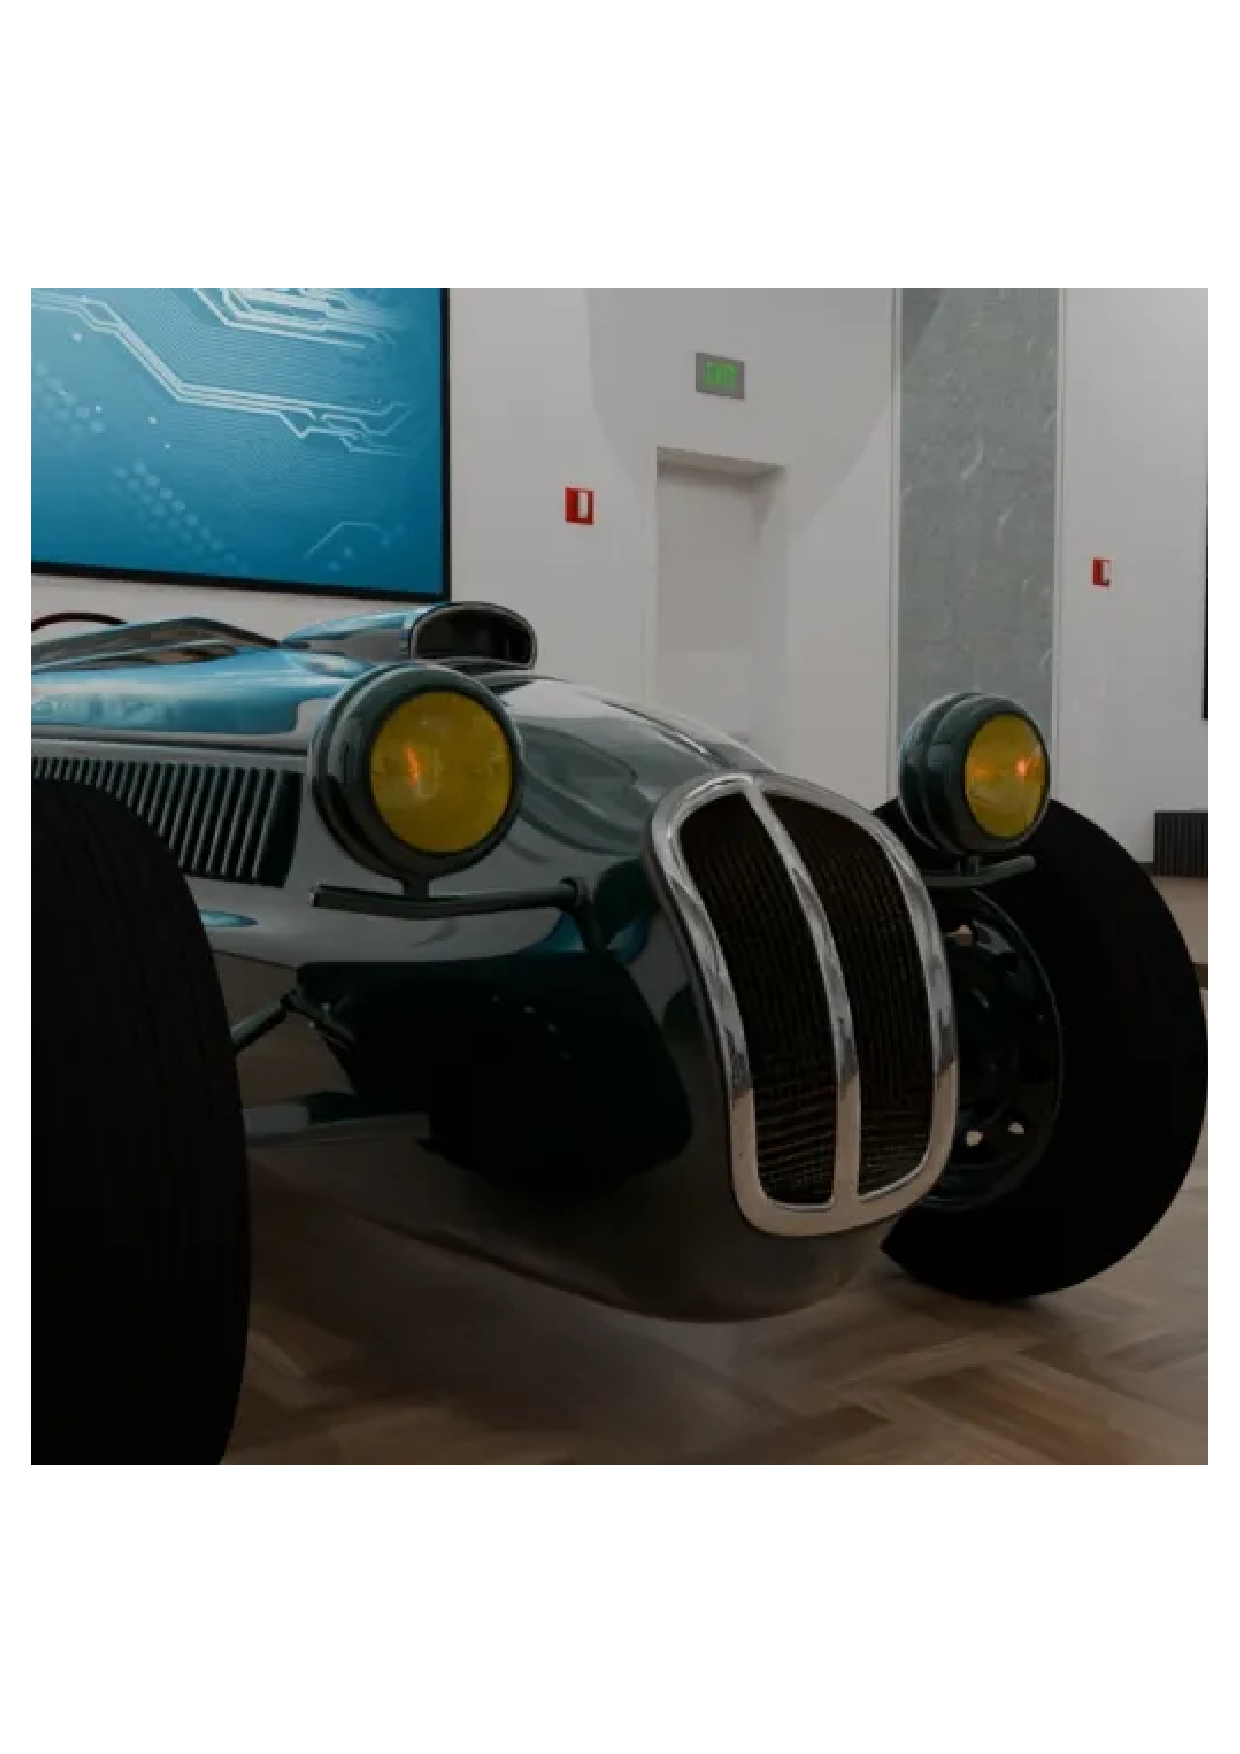
\includegraphics[width=\linewidth]{figures/rightgroundtruthcar.pdf}
    \caption*{Ground Truth}
\end{minipage}
\hfill
\begin{minipage}{0.5\textwidth}
    \centering
    
    \begin{subfigure}{0.48\linewidth}
        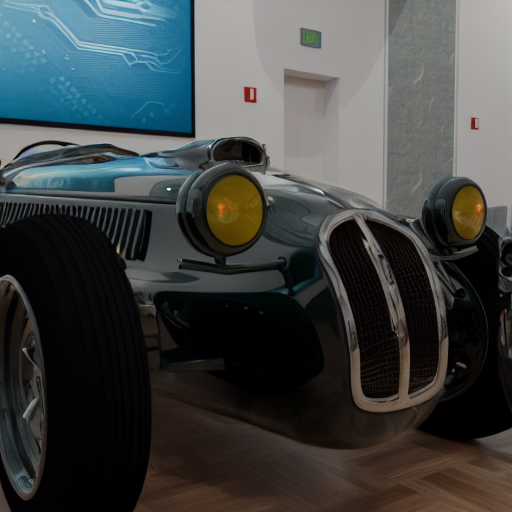
\includegraphics[width=\linewidth]{figures/right_gen2.png}
        \caption*{Eval2}
    \end{subfigure}
    \hfill
    \begin{subfigure}{0.48\linewidth}
        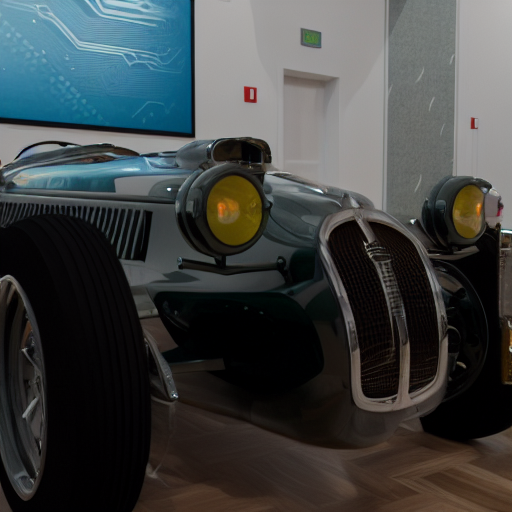
\includegraphics[width=\linewidth]{figures/right_gen3.png}
        \caption*{Eval3}
    \end{subfigure}
    
    \vspace{0.5em}
    
    \begin{subfigure}{0.48\linewidth}
        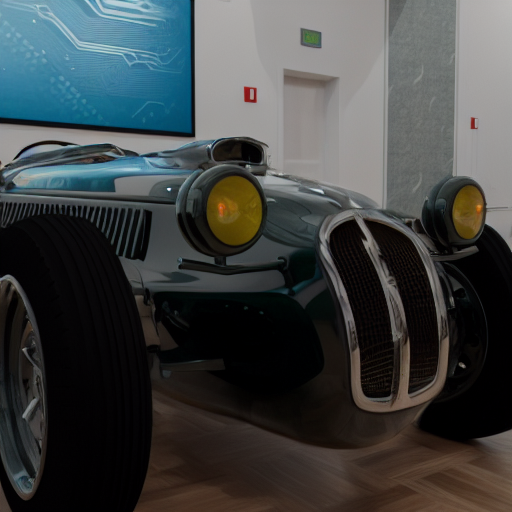
\includegraphics[width=\linewidth]{figures/right_gen4.png}
        \caption*{Eval4}
    \end{subfigure}
    \hfill
    \begin{subfigure}{0.48\linewidth}
        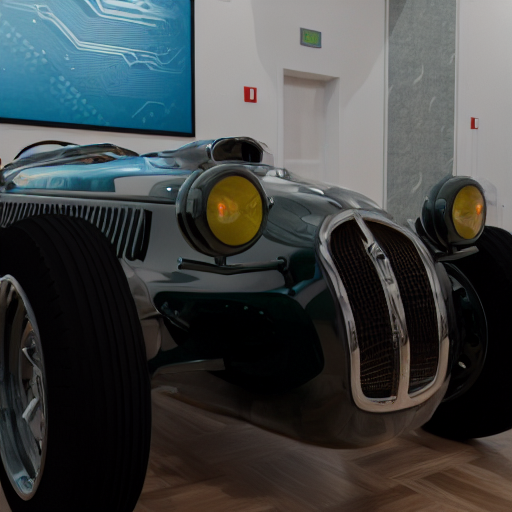
\includegraphics[width=\linewidth]{figures/right_gen8.png}
        \caption*{Eval8}
    \end{subfigure}

\end{minipage}

\caption{Qualitative comparison of generated right-view images. The ground truth image (left) is compared to different evaluation configurations (right).}
\end{figure}

In contrast, the second example (Figure 5) demonstrates a poor representation of the scene, as illustrated by the significant discrepancy of the generated right view images versus the ground truth image. When comparing all of the evaluated configurations (Eval1, Eval4, Eval6 and Eval7) in generating the images of the right view, the models generate structurally inconsistent and partial hallucination results. Although the entire scene appears to represent a dinosaur skeleton, individual bones appear deformed, disconnected or incorrect in their shape, and in several instances the model generates additional structures or removes critical structural components. Due to these failures in maintaining consistency, the alignment of the left and right view images is disrupted and depth relationships become unplausible. These types of errors are even more evident when examining areas with geometric complexity and repetitive structures that indicate that the model has difficulty maintaining consistent disparity in such scenes.

\begin{figure}[H]
\centering

\begin{minipage}{0.45\textwidth}
    \centering
    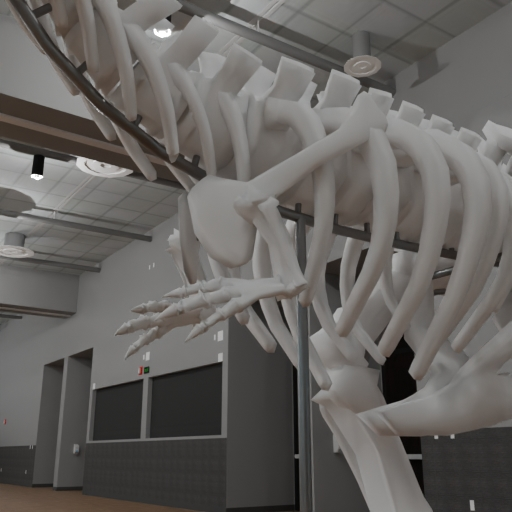
\includegraphics[width=\linewidth]{figures/rightgroundtruthdino.jpg}
    \caption*{Ground Truth}
\end{minipage}
\hfill
\begin{minipage}{0.5\textwidth}
    \centering
    
    \begin{subfigure}{0.48\linewidth}
        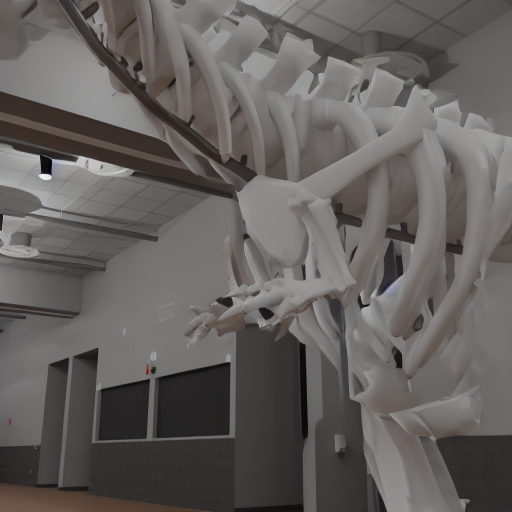
\includegraphics[width=\linewidth]{figures/right_gen1.png}
        \caption*{Eval1}
    \end{subfigure}
    \hfill
    \begin{subfigure}{0.48\linewidth}
        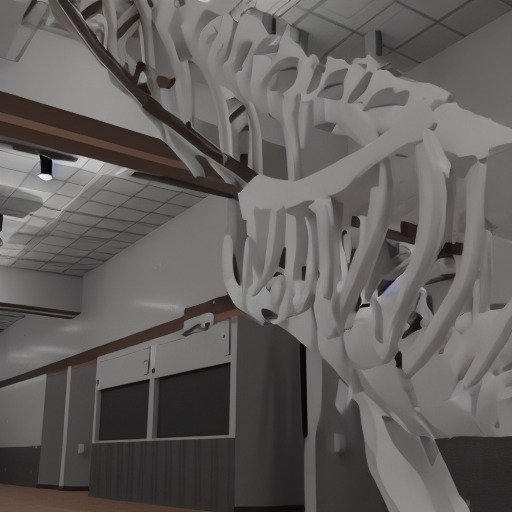
\includegraphics[width=\linewidth]{figures/right_gen44.png}
        \caption*{Eval4}
    \end{subfigure}
    
    \vspace{0.5em}
    
    \begin{subfigure}{0.48\linewidth}
        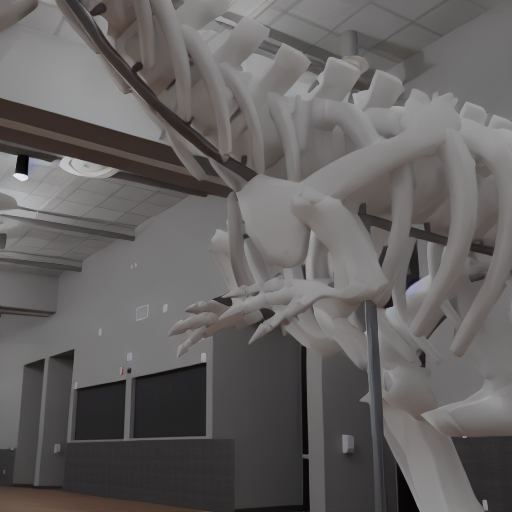
\includegraphics[width=\linewidth]{figures/right_gen6.png}
        \caption*{Eval6}
    \end{subfigure}
    \hfill
    \begin{subfigure}{0.48\linewidth}
        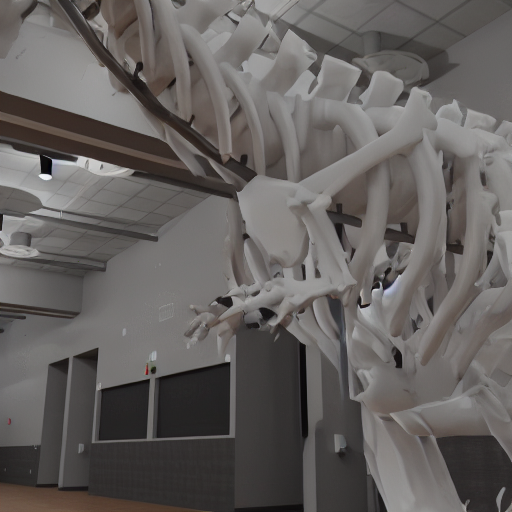
\includegraphics[width=\linewidth]{figures/right_gen7.png}
        \caption*{Eval7}
    \end{subfigure}

\end{minipage}

\caption{Qualitative comparison of generated right-view images. The ground truth image (left) is compared to different evaluation configurations (right).}
\end{figure}

\section{Conclusion}
Our research tested the feasibility of using a training-free method in creating synthetic images from stereo images by testing various different configurations of StereoDiffusion, including evaluating differences within each version of the pipeline.
We found that the first and most basic configuration was able to be replicated and yielded the highest level of quality across all tested versions. We also determined that while an additional depth-based disparity condition does provide another acceptable way of producing similarly good results, there were no improvement in the output quality provided when using either prompt conditioning or more advanced forms of attention mechanisms. Additionally, we demonstrated that both of these conditions typically resulted in decreased levels of stereoscopic consistency.
As such, our study reavels a critical weakness in methods where training is omitted. Specifically, without explicit optimization the inclusion of additional input information will results in diminished performance. As a result, geometric guidance remains the primary factor for achieving high-quality stereo image synthesis.



\section{Future Work}
For our future work we can focus on developing techniques based on training for enabling better and more effective integration of additional conditioned signals such as prompts and depth information. Especially fine tuning this model in stereo-consistent dataset will allow to combine semantics of conditioning signal with geometry constraints which will improve the overall performance. Additionally, use of bigger and more diverse data sets would likely enhance generalization and robustness across different scene types. Evaluation of the developed method at widely used benchmark such as KITTI, will provide a more standardized comparison and help assess cross-dataset performance.
Moreover, studying new architectural alternatives (such as how we design our attentions and how we condition our network) can improve the stability in which we integrate semantic information while maintaining geometric coherence. Evaluating this method against other stereo generative approaches such as Text2Stereo, GenStereo and current 3D aware diffusion models, would give a better understanding of its strengths and limitations.